\documentclass{book}
\usepackage{graphicx}
\usepackage[Export]{adjustbox}
\usepackage{hyperref}

\hypersetup{
    colorlinks=true,
    linkcolor=blue,
    filecolor=magenta,      
    urlcolor=cyan,
    pdftitle={Latihan Soal PSAJ Matematika},
    pdfpagemode=FullScreen,
    }
    
\urlstyle{same}

\begin{document}

\chapter*{Eksponen}

\section*{Sifat Eksponen}

\begin{equation}
\label{ex_mult}
a^{n} \cdot a^{m} = a^{n+m} 
\end{equation}

\begin{equation}
\label{ex_div}
\frac{a^{n}}{a^{m}} = a^{n-m} 
\end{equation}

\begin{equation}
\label{ex_pow}
(a^n)^m = a^{nm}
\end{equation}

\begin{equation}
\label{ex_neg}
a^{-n}=\frac{1}{a^n}
\end{equation}

\begin{equation}
\label{ex_frac}
a^{\frac{n}{m}}=\sqrt[n]{a^m}
\end{equation}

% No. 1
\begin{center}
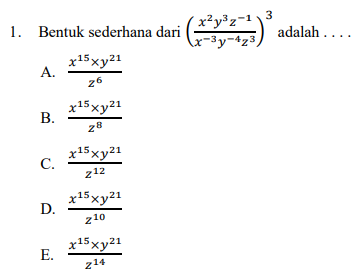
\includegraphics[	valign=t]{1.png} \\
\end{center}
\begin{itemize}
\item[]
Menggunakan sifat eksponen \ref{ex_pow}
\[
	\left(\frac{x^{2}y^{3}z^{-1}}{x^{-3}y^{-4}z^{3}}\right)^3 = \frac{x^{6}y^{9}z^{-3}}{x^{-9}y^{-12}z^{9}}
\]
\item[]
Menggunakan sifat eksponen \ref{ex_neg}
\[
	\frac{x^{6}y^{9}z^{-3}}{x^{-9}y^{-12}z^{9}} =
	\frac{x^{6}y^{9}x^{9}y^{12}}{z^{3}z^{9}}
\]
\item[]
Menggunakan sifat eksponen \ref{ex_mult}
\[
	\frac{x^{6}y^{9}x^{9}y^{12}}{z^{3}z^{9}} = 
	\frac{x^{15} y^{21}}{z^{12}} \left(C\right)
\]
\end{itemize}

% No. 2
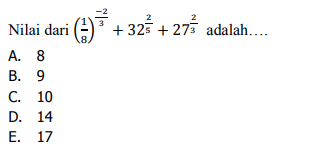
\includegraphics[valign=t]{2.png} \\
Menggunakan sifat eksponen \ref{ex_pow}

\end{document}